\section{Design} \label{chap:design}

Anastasis is a service that allows the user to securely deposit a {\em core
secret} with an open set of escrow providers and recover it if the
secret is lost. The core secret itself is protected from the escrow
providers by encrypting it with a {\em master key}. The main objective of
Anastasis is to ensure that the user can reliably recover the core
secret, while making this difficult for everyone else. Furthermore, Anastasis
supports situations where the user is unable to reliably remember any secret
with sufficiently high entropy, so Anastasis does not simply encrypt using some
other key material in exclusive possession of the user.

To uniquely identify users and to provide a first layer of protection,
an “unforgettable” identifier is used. This identifier should be
difficult to guess for anybody but the user. However, the identifier
is not expected to have sufficient entropy or secrecy to be
cryptographically secure. Examples for such an identifier would be a
concatenation of the full name of the user and their social security
or passport number(s). For Swiss citizens, the AHV number could also
be used.

\subsection{Overview}

The Figure~\ref{fig:legend_keys_anastasis} shows the legend for the
illustration of the Anastasis key usage shown in Figure~\ref{fig:keys_anastasis}
on page~\pageref{fig:keys_anastasis} and in
Figure~\ref{fig:truth_keys} on page~\pageref{fig:truth_keys}.
The Figure~\ref{fig:keys_anastasis} gives an overview of the keys used in Anastasis. It also shows how they are created and used.
Figure~\ref{fig:truth_keys} shows how the keys to sign the (encrypted) truth
data used during authentication are generated. The truth seed(s) used in
Figure~\ref{fig:truth_keys} are part of the recovery document.
\newline
\begin{figure}[H]
	\centering
	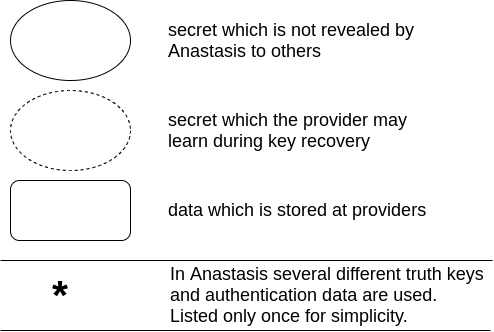
\includegraphics[scale=0.48]{images/legend_keys_anastasis.png}
	\caption{Legend of Figure~\ref{fig:keys_anastasis}} on page~\pageref{fig:keys_anastasis}
	\label{fig:legend_keys_anastasis}
\end{figure}

\begin{figure}[H]
	\centering
	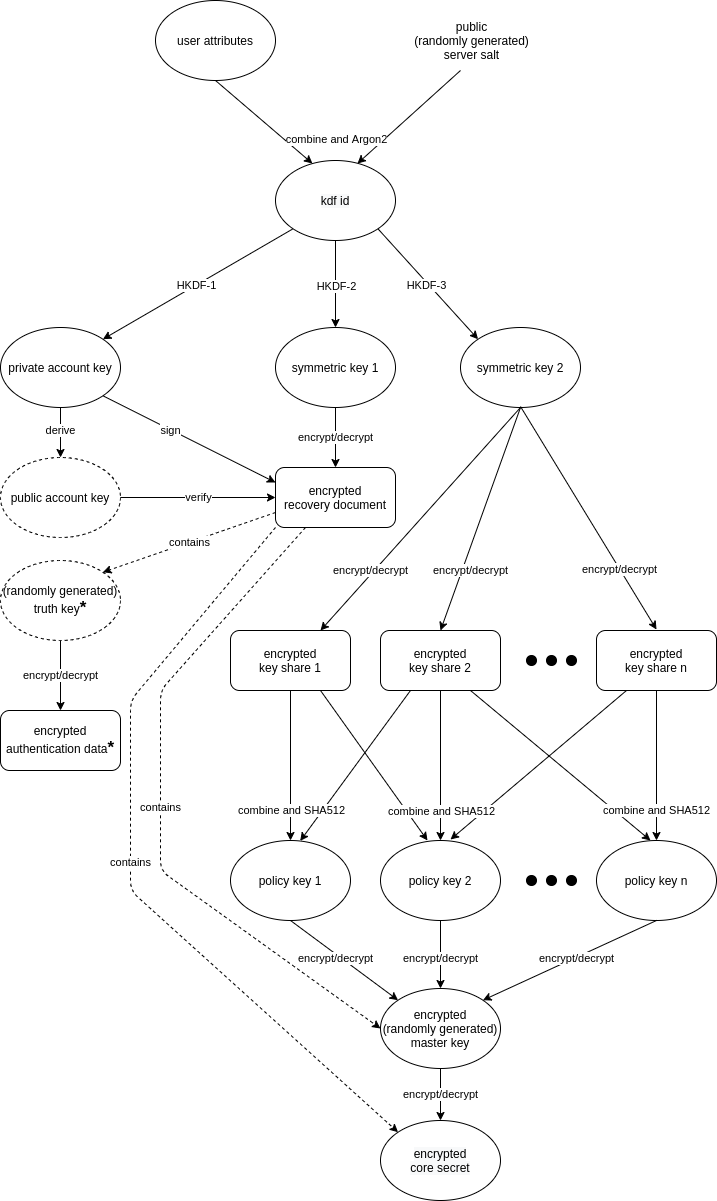
\includegraphics[scale=0.48]{images/keys_anastasis.png}
	\caption{Secrets used in Anastasis}
	\label{fig:keys_anastasis}
\end{figure}

\noindent In the following the keys shown in the Figure~\ref{fig:keys_anastasis} on
page~\pageref{fig:keys_anastasis} are explained:

\begin{description}
	\item[kdf id] {The {\em kdf id} is derived from the user attributes and a
	randomly generated public and constant salt value provided by the escrow provider using Argon2. It is used to derive
	the {\em private account key}, the {\em symmetric key 1} and the {\em symmetric key 2}.}
	\item[private account key] {The {\em private account key} is used to sign the {\em encrypted
	recovery document}. It is derived from the {\em identity key} using {\em HKDF-1}}.
	\item[public account key] {The {\em public account key} is derived from its corresponding
	{\em private account key}. It used to verify the signature of the {\em encrypted recovery
	document} and also is the identifier of the user which is needed by the provider.}
	\item[symmetric key 1] {The {\em symmetric key 1} is derived from the {\em identity key} using
	{\em HKDF-2}. It is used to encrypt and decrypt the {\em encrypted recovery document} which is stored by
	the provider.}
	\item[symmetric key 2] {The {\em symmetric key 2} is derived from the {\em identity key} using
	{\em HKDF-3}. It is used to encrypt and decrypt the different {\em encrypted key shares} which
	are stored by the escrow providers.}
	\item[truth key] {The {\em truth key} is randomly generated for each {\em encrypted authentication data}
	  and is stored within the {\em encrypted recovery document}. It may later be disclosed by the user to
          the escrow provider to let it decrypt the {\em encrypted authentication data} which allows the provider
          to then run the recovery authorization process.}
	\item[master key] {The {\em master key} is randomly generated and is used to encrypt and decrypt the
	{\em encrypted core secret} which is stored within an {\em encrypted recovery document}. The {\em encrypted master key} also is stored within the {\em encrypted recovery document}.}
	\item[policy key] {The {\em policy keys} are used for encryption and decryption of the {\em encrypted master key}. A {\em policy key} is constructed by hashing a specific combination of {\em key shares} specified by the
	user. For hashing SHA512 is used here.}
\end{description}
\newpage

\begin{figure}[H]
	\centering
	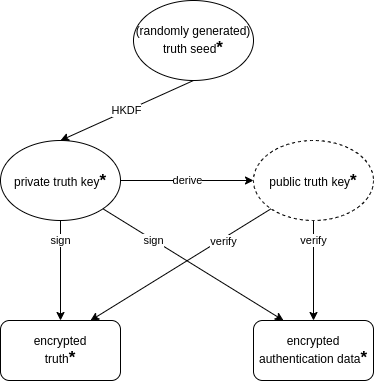
\includegraphics[scale=0.48]{images/truth_anastasis.png}
	\caption{Key generation for signing of encrypted ``Truth'' data in Anastasis}
	\label{fig:truth_keys}
\end{figure}

\noindent In the following the keys shown in the Figure~\ref{fig:truth_keys} on
page~\pageref{fig:truth_keys} are explained:
\begin{description}
\item[truth seed] {Clients generate a random {\em truth seed} for each truth
  which is stored in the encrypted recovery document.}
\item[private truth key] {{\em Private keys} are derived per truth upload. They
  are used to sign the uploaded data. This way, the escrow provider
  can later prove that they preserved the data correctly. We use EdDSA~\cite{josefsson2017} for
  the signatures.}
\item[public truth key] {{\em Public keys} are used to identify the truth
  in the provider's database. Providers only store the first truth upload with
  a valid signature. Changes to truth are thus not possible, clients must
  create a fresh seed for every upload.}
 \end{description}



\subsection{Adversary model}

The adversary model of Anastasis has two types of adversaries: {\em
  weak adversaries} which do not know the user’s identifier (the {\em
  kdf id}), and {\em strong adversaries} which somehow do know a
user’s identifier. Against weak adversaries, the system guarantees
full confidentiality, except for a provider-specific public account
key which links certain requests from the same user, and the data necessary
for authentication. The latter is only disclosed to the providers when
the user requests key recovery. Weak adversaries cannot break
confidentiality even if all escrow providers are part of a conspiracy
of weak adversaries.  For strong adversaries, breaking confidentiality
of the core secret still requires that a sufficient subset of the
Anastasis escrow providers must have colluded with the strong
adversary. The user can specify a set of policies which determine
which Anastasis escrow providers would need to collude to break
confidentiality. These policies also set the bar for the user to
recover their core secret.

Anastasis providers are also not individually trusted to provide
availability or authenticity. Users can specify multiple policies, and
satisfying any one of the policies would allow them to recover their
core secret assuming the subset of providers specified in the policy
is available (and preserved the authenticity of the data).  As clients
sign their uploads, they can verify the authenticity of the data
returned by checking the signatures.  Only strong adversaries are able
to forge signatures, so they could create fraudulent recovery
documents and/or key shares resulting in invalid restored core
secrets. However, because uploads are never destructive, strong
adversaries can only succeed in breaking availability if they collude
with a subset of escrow providers that are present in all policies
selected by the user.

Thus, users can improve confidentiality by having many different
escrow providers in their policies, and improve availability by having
many policies with few escrow providers. Anastasis does not resolve
this trade-off, but allows users to make individual choices and gives
them agility with respect to the parties whom they offer their
trust, resulting in trust agility~\cite{marlinspike2011}.


\subsection{Encryption of the core secret}

The {\em core secret} of the user is (AES)~\cite{heron2009} encrypted using a symmetric
{\em master key}.  Recovering the master key requires the user to
satisfy a {\em policy}. Policies specify a set of escrow methods, each
of which leads the user to a {\em key share}. Combining those key
shares (by hashing) allows the user to obtain a policy key, which can
be used to decrypt the master key.  There can be many policies,
satisfying any of these will allow the user to recover the master key.

Which escrow methods are combined into which policies and which
providers are involved can be different for each user. As users are
unlikely to remember all the details, Anastasis needs a way to
remember the specific configuration a user made.

This process description is provided in a {\em recovery document}.

% Figure~\ref{fig:recoverydoc} gives an example for a the contents of
% a recovery document.
% FIXME: actually include example!


\subsection{The recovery document}

A {\em recovery document} includes all the information a user needs to
recover access to their core secret. It primarily identifies a set of
{\em encrypted key shares} which have been entrusted to different
Anastasis providers. For each key share, the recovery document
specifies the respective Anastasis provider and also prescribes the
{\em authentication method}, which specifies how the user should
convince the Anastasis server that they are authorized to retrieve the
encrypted key share.  Authentication methods can for example include
SMS-based verification, video-identification or a security question.

For each authentication method, specific Anastasis providers are separately
provided (see Section~\ref{sec:truth}) with the associated {\em encrypted key
  share} and (separately encrypted) {\em authentication
  data}. Anastasis operators may learn the authentication data during
the recovery process to authenticate the user. Examples for
authentication data would be a phone number (for SMS), a picture of
the user (for video identification), or the (hash of) a security
answer. A strong adversary is assumed to be able to learn the
authentication data, while weak adversaries must not (except if they
are the provider and then they may learn it only during key recovery).

The recovery document also specifies {\em policies}, which describe
the combination(s) of the key shares (and thus authentication
processes) that would suffice to obtain access to the core secret. For
example, a policy could say that the authentication methods ``$A$ and
$B$'' suffice, and a second policy may permit ``$A$ and $C$''. A
different user may choose to use the policy that ``$A$ and $B$ and
$C$'' are all required. Anastasis imposes no limit on the number of
policies in a recovery document, or the set of providers or
authentication methods involved in guarding a user’s secret.

Weak adversaries must not be able to deduce information about a user’s
recovery document (except for meta data such as its length or
approximate creation time, which may be exposed to an adversary which
monitors the user’s network traffic or operates an escrow provider).


\subsection{Identity-derived encryption}

To start, a user provides their private (alas not really secret),
unique and unforgettable user attributes as a seed to identify their
account. For example, this could be a social security number together
with their full name. Specifics may depend on the cultural context, in
this document we will simply refer to this information as the
{\em user attributes}.

For each Anastasis provider, a {\em kdf id} key is derived from the
user’s attributes and a provider salt using Argon2~\cite{BDK2016}, a
computationally expensive cryptographic hash function. Using an
expensive hash algorithm is assumed to make it harder for a weak
adversary to determine user attributes by brute force guessing.  The
salt ensures that the keys for the same user cannot be easily
correlated across the various Anastasis servers.  However, it is
assumed that a strong adversary performing a targeted attack can
compute the {\em kdf id}s.

The listing in Figure~\ref{fig:argon2} provides pseudo-code for
the computation of the {\em kdf id}. The inputs are:

\begin{description}
	\item[attributes] {The personal attributes provided by the user.}
	\item[server\_salt]{The salt from the Anastasis provider.}
	\item[keysize]{The desired output size of the KDF, here 32 bytes.}
\end{description}

\begin{figure}[H]
\begin{lstlisting}
user_identifier_derive(attributes, server_salt, keysize)
{
  kdf_id = Argon2(attributes, server_salt, keysize)
  return kdf_id
}
\end{lstlisting}
\caption[Use of Argon2 to derive user attributes]{The user's attributes are hashed with Argon2, to provide a
  kdf\_id which will be used to derive other keys later. The hash must
  also be made over the respective provider's server\_salt. This
  ensures that the kdf\_id is different on each server. The use of
  Argon2 and the respective server\_salt are intended to make it
  difficult to brute-force kdf\_id values and help protect user’s
  privacy. Also this ensures that the kdf\_ids on every server
  differs. However, we do not assume that the identifier or the
  kdf\_id cannot be determined by an adversary performing a targeted
  attack, as a user’s identifier is likely to always be known to state
  actors and may likely also be available to other actors.}
\label{fig:argon2}
\end{figure}

Anastasis derives symmetric key material --- but not the master secret --- from the {\em kdf id} using different HKDFs~\cite{krawczyk2010}.

When confidential data --- such as the recovery document or the truth
--- is uploaded to an Anastasis server, the respective payload is
encrypted using AES-GCM with the respective symmetric key and
initialization vector derived key material as shown in
Figure~\ref{fig:keys_anastasis} and a high-entropy nonce.  The nonce
and the GCM tag are prepended to the ciphertext before being uploaded
to the Anastasis server. This is done whenever confidential data is
stored with the server, so both for encrypted authentication data
(\texttt{/truth} uploads) and encrypted recovery documents
(\texttt{/policy} uploads).

To ensure that the key derivation for the encryption of the recovery
document differs fundamentally from that of an individual key share,
we use different salts for different types of operations (“erd” and
“eks” respectively):

\begin{lstlisting}
encryption_key_create(kdf_id, salt, nonce)
{
iv, key = HKDF (kdf_id, nonce, salt, keysize + ivsize)
return iv,key
}
\end{lstlisting}

\begin{description}
	\item[HKDF()] {The HKDF-function uses to phases: First we use HMAC-SHA512 for the extraction phase, then HMAC-SHA256 is used for expansion phase.}
	\item[kdf\_id] {Hashed identifier.}
	\item[keysize] {Size of the AES symmetric key, here 32 bytes.}
	\item[ivsize] {Size of the AES GCM IV, here 12 bytes.}
	\item[nonce] {32-byte nonce, must never match “ver” (which it cannot as the length is different). Of course, we must avoid key reuse. So, we must use different nonces to get different keys and ivs (see below).}
	\item[key] {Symmetric key which is later used to encrypt the documents with AES256-GCM.}
	\item[iv] {IV which will be used for AES-GCM.}
\end{description}


\begin{lstlisting}
encrypt(kdf_id, data, salt)
{
nonce = generate_random_bytes(32)
iv, key = encryption_key_create(kdf_id, salt, nonce)
encrypted_data, aes_gcm_tag =  AES256_GCM(data, iv, key)
encrypted_data = nonce + aes_gcm_tag + encrypted_data
return encrypted_data
}

key_share_encrypt(kdf_id, key_share)
{
encrypted_key_share = encrypt(kdf_id, key_share, "eks")
return encrypted_key_share
}

recovery_document_encrypt(kdf_id, recovery_document)
{
encrypted_recovery_document =
encrypt(kdf_id, recovery_document, "erd")
return encrypted_recovery_document
}

\end{lstlisting}

\begin{description}
	\item[encrypted\_recovery\_document] {The encrypted recovery document which contains the authentication methods, policies and the encrypted core secret.}
	\item[encrypted\_key\_share] {The encrypted key\_share which the escrow provider must release upon successful authentication.}
	\item[nonce] {Nonce which is used to generate keys and ivs which are used for the encryption. The nonce must contain either eks or erd.}
	\item[encrypted\_data] {The encrypted data contains the either a recovery document or a key share which was encrypted and the nonce and the aes\_gcm\_tag. To be able to decrypt it the first 32 Bytes are the nonce and the next 12 Bytes are the aes\_gcm\_tag.}
\end{description}


\subsection{Authenticity of recovery documents}

\texttt{/policy/} requests are used to upload new encrypted recovery
documents. For users to authorize \texttt{/policy} operations, we need
an account key pair.  Thus, in addition to the symmetric keys, an
EdDSA-based {\em account key} is derived from the {\em kdf id} (see
Figure~\ref{fig:keys_anastasis}) and used to identify the ``account''
of the user at each Anastasis server.  EdDSA public keys are always
points on Curve25519 and represented using the standard 256-bit
Ed25519 compact format. The binary representation is converted to
Crockford Base32 when transmitted inside JSON or as part of URLs in
the RESTful API of Anastasis (see Section~\ref{sec:serverarch}).
EdDSA signatures are also provided in Crockford Base32-encoding and
transmitted using the HTTP header
\texttt{Anastasis-Account-Signature}.  Encrypted recovery documents
are stored using the public account key as the identifier.

As the account keys are derived from the {\em kdf id} --- which strong
adversaries are assumed to know ---, we cannot assure that the corresponding
private account key is truly secret. Thus, policy operations must
never be destructive: A strong adversary can derive the private key
and access (and with the {\em kdf id} also decrypt) the user’s
recovery document (but not the core secret!), and also upload a new
version of the encrypted recovery document. However, because uploads
are not destructive, even a strong adversary cannot delete an existing
version and thus cannot break availability.

For the generation of the private key we use the {\em kdf id} as the
entropy source, hash it to derive a base secret which will then be
processed to fit the requirements for EdDSA private keys. From the
private key we can then generate the corresponding public key. Here,
the string “ver” is used for the salt value for the HKDF to ensure
that the result differs from other cases where we hash {\em kdf id}:

\begin{lstlisting}
eddsa_keys_create (kdf_id, salt, keysize)
{
  ver_secret = HKDF(kdf_id, salt, keysize)
  eddsa_priv = ver_secret
  eddsa_pub = get_eddsa_pub(eddsa_priv)
  return eddsa_priv, eddsa_pub
}
\end{lstlisting}

\begin{description}
	\item[HKDF()] {The HKDF-function uses to phases: First we use HMAC-SHA512 for the extraction phase, then HMAC-SHA256 is used for expansion phase.}
	\item[kdf\_id] {Hashed identifier.}
	\item[salt] {Is used that different keys are generated, the salt here is "ver".}
	\item[key\_size] {Size of the output, here 32 bytes.}
	\item[ver\_secret] {Derived key from the kdf\_id, serves as intermediate step for the generation of the private key.}
\end{description}

\begin{description}
	\item[eddsa\_priv] {The generated EdDSA private key.}
	\item[eddsa\_pub] {The generated EdDSA public key.}
\end{description}


\subsection{Account signatures}

The EdDSA account keys are used to sign the encrypted recovery
document sent from the client to the server.

% FIXME: "everything"? I don't think we can sign the encrypted truth
% with the eddsa_priv, as that would link the truth to the ERD.
% We need ANOTHER account key here, one per truth + provider?

\begin{lstlisting}
(anastasis-account-signature) = eddsa_sign(h_body, eddsa_priv)
ver_res =
  eddsa_verifiy(h_body, anastasis-account-signature, eddsa_pub)
\end{lstlisting}

\begin{description}
	\item[anastasis-account-signature] {Signature over the SHA-512 hash of the body using the purpose code TALER\_SIGNATURE\_ANASTASIS\_POLICY\_UPLOAD (1400) (see GNUnet EdDSA signature API for the use of purpose).}
	\item[h\_body] {The hashed body.}
	\item[ver\_res] {A Boolean value. True: Signature verification passed, False: Signature verification failed.}
\end{description}

\noindent
When requesting \texttt{/policy} downloads, the client must also provide a signature:
\begin{lstlisting}
(anastasis-account-signature) = eddsa_sign(version, eddsa_priv)
ver_res =
  eddsa_verifiy(version, anastasis-account-signature, eddsa_pub)
\end{lstlisting}

\begin{description}
	\item[anastasis-account-signature] {Signature over the SHA-512 hash of the body using the purpose code TALER\_SIGNATURE\_ANASTASIS\_POLICY\_DOWNLOAD  \\
	(1401) (see GNUnet EdDSA signature API for the use of purpose).}
	\item[version] {The version requested as a 64-bit integer, for the “latest version”.}
	\item[ver\_res] {A Boolean value. True: Signature verification passed, False: Signature verification failed.}
\end{description}


\subsection{Authenticity of truth} \label{sec:truth}

\texttt{/truth/} requests are used to upload encrypted authentication data
and encrypted key shares to an Anastasis escrow service.  As an additional
layer of protection, an Anastasis escrow service cannot link truth data to
policy data, except maybe by observing the timing of the requests.

Anastasis uses EdDSA-based {\em truth key}s to identify truth
objects. For those, the truth keys are derived from a {\em truth
  seed}, as show in Figure~\ref{fig:truth_keys}.  The private truth
key is used to authorize the truth upload. The signatures also
authenticate the encrypted key shares returned from the Anastasis
provider during recovery.  The signature process for truth is
analogous to that for accounts.


\subsection{Availability considerations}

Anastasis considers two main threats against availability. First, the
Anastasis server operators must be protected against denial-of-service
attacks where an adversary attempts to exhaust operator’s
resources. The API protects against these attacks by allowing
operators to set fees for expensive operations. Furthermore, all data stored
comes with an expiration logic, so an attacker cannot force servers to
store data indefinitely.

A second availability issue arises from strong adversaries that may be
able to compute the account keys of some user. While we assume that
such an adversary cannot successfully authenticate against the truth,
the account key does inherently enable these adversaries to upload a
new policy for the account. This cannot be prevented, as the
legitimate user must be able to set or change a policy using only the
account key. To ensure that an adversary cannot exploit this, policy
uploads first of all never delete existing policies, but merely create
another version. This way, even if an adversary uploads a malicious
policy, a user can still retrieve an older version of the policy to
recover access to their data. This append-only storage for policies
still leaves a strong adversary with the option of uploading many
policies to exhaust the Anastasis server’s capacity. We limit this
attack by requiring a policy upload to include a reference to a
payment identifier from a payment made by the user. Thus, a policy
upload requires both knowledge of the identity and making a
payment. This effectively prevents and adversary from using the
append-only policy storage from exhausting Anastasis server capacity.
